% ----------------------- TODO ---------------------------
% Diese Daten müssen pro Blatt angepasst werden:
\newcommand{\NUMBER}{VHDL Vorführung}
\newcommand{\EXERCISES}{5}
% Diese Daten müssen einmalig pro Vorlesung angepasst werden:
\newcommand{\COURSE}{Grundlagen der Digitaltechnik}
\newcommand{\TOPIC}{}
\newcommand{\DATE}{10.06.2022}
% ----------------------- TODO ---------------------------

\documentclass[a4paper]{scrartcl}

\usepackage[utf8]{inputenc}
\usepackage[ngerman]{babel}
\usepackage{amsmath}
\usepackage{amssymb}
\usepackage{fancyhdr}
\usepackage{color}
\usepackage{graphicx}
\usepackage{lastpage}
\usepackage{listings}
\usepackage{tikz}
\usepackage{pdflscape}
\usepackage{subfigure}
\usepackage{float}
\usepackage{polynom}
\usepackage{hyperref}
\usepackage{tabularx}
\usepackage{forloop}
\usepackage{geometry}
\usepackage{listings}
\usepackage{fancybox}
\usepackage{tikz}
\usepackage{algpseudocode,algorithm,algorithmicx}

%Definiere Let-Command für algorithmen
\newcommand*\Let[2]{\State #1 $\gets$ #2}

\input kvmacros

%Größe der Ränder setzen
\geometry{a4paper,left=3cm, right=3cm, top=3cm, bottom=3cm}

%Kopf- und Fußzeile
\pagestyle {fancy}
\fancyhead[L]{\COURSE}
\fancyhead[R]{\DATE}

\fancyfoot[L]{}
\fancyfoot[C]{}
\fancyfoot[R]{Seite \thepage /\pageref*{LastPage}}
\setlength{\parindent}{0pt}

%Formatierung der Überschrift, hier nichts ändern
\def\header#1#2{
  \begin{center}
    {\Large Labor: #1 \TOPIC}\\
    {(Datum #2)}
  \end{center}
}


\begin{document}


\header{ \NUMBER}{\DATE}


\section*{Aufgabe 1: Full-Adder Beispiel}
\subsection*{a) Simulation}
Das Beispiel besteht aus zwei Dateien. In \texttt{adder.vhd} ist der eigentliche 1-Bit Full-Adder implementiert. 
Schaue in den Code versuche zu verstehen was dort passiert. \\
In \texttt{tb\_adder.vhd} ist die Testbench für die Schaltung. Mit ihrer Hilfe kann man den Full-Adder simulieren und wir können die Funktionalität überprüfen.
Verusche nachzuvollziehen wie die Testbench mit der adder-Entity verschalten ist und was mit den Signalen der Testbench passiert. Warum hat die Testbench kein I/O?\\

Für die Simulation kann unter Linux einfach das mitgelieferte Makefile ausgeführt werden. Für Windows/MacOS muss ein Script mit den folgenden Commands angelegt werden (PathToExe 
wird jeweils nicht benötigt, wenn Executables in der Pfad Variable eingetragen wurden). Stelle sicher, dass die Befehle im Verzeichnis des VHDL-Projekts ausgeführt wird:\\
Windows:
\begin{itemize}
  \item $<$PathToExe$>$/ghdl -a --std=08 adder.vhd tb\_adder.vhd
	\item $<$PathToExe$>$/ghdl -e --std=08 adder\_tb
	\item $<$PathToExe$>$/ghdl -r --std=08 adder\_tb --wave=wave.ghw --stop-time=50ns
	\item $<$PathToExe$>$/gtkwave wave.ghw
\end{itemize}
Linux:
\begin{itemize}
  \item make
	\item gtkwave wave.ghw
\end{itemize}

Mit dem \texttt{gtkwave} Befehl sollte ein Fenster aufgegangen sein, in welchem man nun die Simulationsergebnisse anschauen kann.
\begin{figure}[h]
  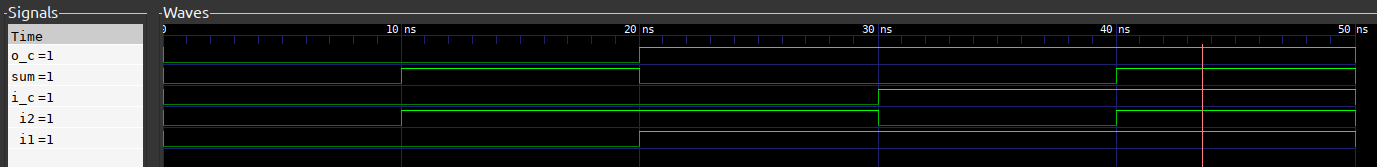
\includegraphics[width=\textwidth]{gtkwave.png}
\end{figure}

Tut der Adder was er soll?

\subsection*{b) Design vs. Simulation}
Mit dem GHDL-Compiler kann man zwar seine VHDL Designs simulieren, aber man kann damit keine Binär-Files erzugen, die man zum Beispiel in ein FPGA programmieren kann. 
Um aus einem VHDL Design eine Datei zu erzeugen, welche in ein FPGA geladen werden kann, benötigt man meist eine Design IDE des Herstellers (z.B. Xilinx Vivado o.
Intel Quartus). Diese IDEs integrieren meist direkt einen Simulator, so dass man in einer großen IDE entwickeln, simulieren und das Binär-File erstellen kann. Diese
Suites sind typischerweise mehrere Gigabyte groß und sind meist nicht umsonst.

\subsection*{c) To Be Synthesizeable or Not To Be Synthesizeable}
Synthesizeable (oder synthethisierbar) bedeutet das Design (der VHDL Code) in eine niedrigere Abstraktionschicht zu bringen (z.B. aus VHDL nach RTL (Register Transfer Logik)). Dies wird
benötigt, um aus einem Design letzten Endes Lithografiemasken für einen Chip oder das Binär-File für ein FPGA zu erzeugen. 

Versuche zu verstehen warum die adder-Entity in \texttt{adder.vhd} synthethisierbar ist (bedeutet die könnten wir ``in'' ein FPGA/Chip bringen), die Testbench (tb) aber nicht.
Das bedeutet die Testbench kann lediglich für die Simulation hergenommen werden.

\section*{Aufgabe 2: Der 3 Bit-Adder}
Versuche mit der 1-Bit Adder Komponente durch Verschaltung einen 3-Bit Adder zu erstellen. Erstelle auch hier für eine Testbench und für eine Simulation durch.

\section*{Aufgabe 3: ALU (Bonusaufgabe für Zuhause)}
Modelliere und simuliere die ALU aus Labor 2 mit VHDL. Gehe hier Schritt für Schritt vor:\\
\begin{itemize}
  \item Erstelle Entities für jeden Block (z.B. für das 8-Bit OR).
  \item Erstelle Testbenches für jeden Block
  \item Simuliere/Teste jeden einzelnen Block auf korrekte Verschaltung
  \item Verschalte die Blöcke in einer Top-Level Entity
  \item Erstelle eine Testbench für die Top-Level Entity und simuliere diese
\end{itemize}


\end{document}
%%% Local Variables:
%%% mode: latex
%%% TeX-master: t
%%% End: